\chapter{Visualization}\label{chap:visualization}

\vampire provides tools for visualising systems using external programs such as Rasmol, Jmol and POV-Ray. To compile these utilities, use the following command in the main directory of your \vampire installation folder:

\noindent
\begin{minipage}[c]{\textwidth}
\centering
\textit{make vdc}
\end{minipage}

The \vampire data converter, or \vdc, is run to produce the input files needed. To generate the input files, an output type must be specified in the command line. For example, to produce POV-Ray input files:

\noindent
\begin{minipage}[c]{\textwidth}
\centering
\textit{vdc -{}-povray}
\end{minipage}

Note that all command line parameters passed to vdc are not case sensitive.

\section*{Getting started}
\phantomsection\addcontentsline{toc}{section}{Getting started}

To generate the positions of your atoms, \textit{config:atoms} must be set in the input file. This will produce .data and .meta files containing the atomic and spin configuration of your system. Their frequency can be adjusted using the \textit{config:atoms-output-rate} paramter or they can be set to be output at the end of the simulation solely.

In addition, the format of the output can be text or binary format, the latter can help with particulary large systems. Files written in binary format are system specific and usually cannot be read by \vdc compiled on separate hardware.

\subsection*{input}
{\footnotesize
\begin{verbatim}
#------------------------------------------
# data output
#------------------------------------------
config:atoms
config:output-nodes      = 12
config:atoms-output-rate = 1000
config:output-format     = binary
\end{verbatim}
}

\section*{Atomic visualization with rasmol}
\phantomsection\addcontentsline{toc}{section}{Atomic visualization with rasmol}

To visualise your system using Rasmol, simply run \vdc in the same directory as your output with \textit{vdc -{}-xyz}. The \textit{config:atoms} files must be present.

This produced a file called \textit{crystal.xyz}, which is a chemical file format with information on the atomic positions. The format of the \textit{.xyz} format is as follows:

\subsection*{.xyz}
{\footnotesize
\begin{verbatim}
<number of atoms>
comment line
<element> <X> <Y> <Z>
...
\end{verbatim}
}

The element in the .xyz file does not necessarily need to be the same as the atoms used in your system. They can instead be chosen for a different colour palette depending on the users requirements.

\section*{Atomic visualization with POV-Ray}
\phantomsection\addcontentsline{toc}{section}{Atomic visualization with POV-Ray}

To produce pictures of your material of punishable quality and high configurability, it is also possible to use POV-Ray. After running \vdc, the file "spins.pov" contains all the necessary information and an image may be produced by using:

\noindent
\begin{minipage}[c]{\textwidth}
\centering
\textit{povray spins.pov}
\end{minipage}

When running povray it is also possible to select specific snapshots or ranges to render using the following flags:

\noindent
\begin{minipage}[c]{\textwidth}
\centering
\textit{povray +KFF[initial frame number] +KFI[final frame number]}
\end{minipage}

For example, to render frame 9 only, you could use:

\noindent
\begin{minipage}[c]{\textwidth}
\centering
\textit{povray -W3600 -H2700 +A0.3 +KFI9 +KFF9 spins.pov}
\end{minipage}

\noindent where the "-W" and "-H" flags define the width and heigh of the image (the resolution), and "+A" is used for antialiasing.

Output from \vdc can be customised in several ways, either by passing parameters to the command line (using the '\textit{--}' notation), or by using a separate \vdc input file. The \vdc input file is a plain text file containing parameters and arguments which change the output behaviour. This should be helpful when many parameters, or multiple vdc runs with the same parameters, are needed. Comments can be included with the '\#' symbol and the special characters ' ,()\{\}[]:=!' can also be used but are ignored by \vdc.  By default this file is called \textit{vdc-input}, and is read automatically. To change the name of the \vdc input file, a command line parameter can be used:

\noindent
\begin{minipage}[c]{\textwidth}
\centering
\textit{vdc -{}-input-file [filename]}
\end{minipage}

There are many options that can be used to change all visualisation outputs including Rasmol, Jmol and POV-Ray. To get help with the usage of these parameters outside of the manual, it is also possible to print help messages from the command line by using the \textit{-h} or \textit{-{}-help} command line argument, followed by the name of a \textit{vdc-input} file parameter:

\noindent
\begin{minipage}[c]{\textwidth}
\centering
\textit{vdc -h [parameter-name]}
\end{minipage}

The help message should contain information on the parameter, as well as the type of the associated value given, the default value and example usage of the parameter.

\section*{General customisation options}
\phantomsection\addcontentsline{toc}{section}{General Customisation options}

It may be beneficial to use only smaller portions of your full system when generating POV-Ray or Rasmol images. This can help with large systems where rendering can become a time constraint, or systems made up of several elements which might be less relevant for the visualisation. There are several similar command line options which can be used to cut up the system in different ways:

{\zicf slice = float vector(6) [0-1 : default \{0,1,0,1,0,1\}]}\phantomsection\addcontentsline{toc}{subsection}{slice} The first slice type defines minimum and maximum values for each axis. Only atoms and spins inside these boundaries are included in the visualisation. The parameters passed to this argument are interpreted as fractional coordinates.

{\zicf slice-void = float vector(6) [0-1 : default \textit{not set}]}\phantomsection\addcontentsline{toc}{subsection}{slice-void} This parameter will \textit{remove} all atoms and spins inside the given borders. This can be used to create cubic hollow systems where only surface atoms are shown,  removing a very high percentage of atoms in the system, which can greatly reduce rendering time for both POV-Ray and Rasmol. 

{\zicf slice-sphere = float vector(3) [0-1 : \textit{xfrac},\textit{yfrac},\textit{zfrac}]}\phantomsection\addcontentsline{toc}{subsection}{slice-sphere} The sphere slice is also used to remove the atoms and spins at the centre of a system. This particular parameter lends itself well to spherical systems as it removes a spherical section of atoms. Three parameters are required, instead of six. Each one defines a region, centred on the centre of the original system, along the respective axis, equal to a fraction of the system size along that axis. As these parameters are not necessarily equal to each other, this can be used to create an ellipse of missing atoms at the centre of the system.

{\zicf slice-cylinder = float vector(4) [0-1 : \textit{xfrac},\textit{yfrac},\textit{zmin},\textit{zmax}]}\phantomsection\addcontentsline{toc}{subsection}{slice-cylinder} This slice parameter can be used to remove all atoms outside a cylindracal section by defining the x,y-fractional sizes as well as a fractional minimum and maximum along the z-axis.

{\zicf remove-materials = int [one or more values] }\phantomsection\addcontentsline{toc}{subsection}{remove-materials} In some cases whole materials are not relevant for visualisation purposes and can be altogether removed. To use this command line parameter a list of material indices need to be provided. Material indices start from 1.

\section*{POV-Ray Customisation options}
\phantomsection\addcontentsline{toc}{section}{POV-Ray Customisation options}

The following section contains a list of parameters that only affect POV-Ray output configurations. If another output type is requested, these parameters are ignored.

{\zicf frame-start = int [default 0]}\phantomsection\addcontentsline{toc}{subsection}{frame-start} Depending on output options used in \vampire, multiple frames may be rendered by \vdc. \textit{frame-start} can be used to skip an initial number of frames.

{\zicf frame-final = int [default 0]}\phantomsection\addcontentsline{toc}{subsection}{frame-final} Depending on output options used in \vampire, multiple frames may be rendered by \vdc. \textit{frame-final} can be used to skip later frames.

{\zicf camera-position = float vector(3) [(-1,1) : default \textit{not set}]}\phantomsection\addcontentsline{toc}{subsection}{camera-position} POV-Ray camera position, set using fractional coordinates. Camera distance from look at point is calculated automatically however it can be changed by using \textit{camera-zoom}.

{\zicf camera-look-at = float vector(3) [(-1,1) : default \textit{not set}]}\phantomsection\addcontentsline{toc}{subsection}{camera-look-at} POV-Ray camera look at position, set using fractional coordinates. The position is a location in the bounding box of the system, with centre (0,0,0).

{\zicf camera-zoom = float vector(3) [0-$\infty$ : default \textit{not set}]}\phantomsection\addcontentsline{toc}{subsection}{camera-zoom} The default distance from the camera is automatically calculated according to the size of the system. This can be increased or reduced using \textit{camera-zoom} to multiply the default distance. Values less than 1.0 reduce the distance while values above 1.0 increase it.

{\zicf background-colour = string [default Gray30]}\phantomsection\addcontentsline{toc}{subsection}{background-colour} POV-Ray includes various predefined colours such as \textit{White, Black, Gray}. Misspelled colour names will not be detected by vdc but will cause error in POV-Ray.

{\zicf atom-sizes = float [one or more : default 1.2]}\phantomsection\addcontentsline{toc}{subsection}{atom-sizes} POV-Ray atom sizes. Atoms are represented by spheres with a defined radius. Individual materials can have different atoms sizes by including a list of floats, starting from material 1.

{\zicf arrow-sizes = float [one or more : default 2.0]}\phantomsection\addcontentsline{toc}{subsection}{arrow-sizes} POV-Ray arrow sizes. Individual materials can have different arrow sizes by including a list of floats, starting from material 1.

\begin{figure*}[!h]
\center
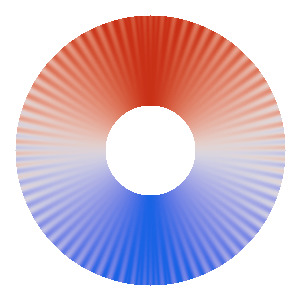
\includegraphics[width=4cm]{figures/CBWR_colourmap.jpg}
\\ CBWR colourmap
\label{fig:CBWR_colourmap}
\end{figure*}

{\zicf colourmap = string [default CBWR]}\phantomsection\addcontentsline{toc}{subsection}{colourmap} By default, a 1D colourmap is used. Aligned along the z-axis, spins in the \{0,0,1\} direction are red, while spins antiparallel to this \{0,0,-1\} are blue. Between these values, the colour transitions to white around the xy-plane. This corresponds to the \textit{CBWR} colourmap, a cyclic blue-white-red map, which lends itself well to 1D or 2D spin sytems where there are two principle spin directions, such as antiferromagnets and ferrimagnets. Some care must be taken to align the principle spin directions with the z-axis, as this is the axis along which colour is applied. This can also be changed using the \textit{vector-z} input parameter. There are several choices of possible colourmap configurations, the ones provided by default are made to be perceptually uniform and in some cases take account of colourblindness. Information on the colourmaps, the importance of perceptually uniform maps and how to adapt and use different maps can be found from \textit{"Peter Kovesi. Good Colour Maps: How to Design Them. 2015"}.

\begin{figure*}[!h]
\center
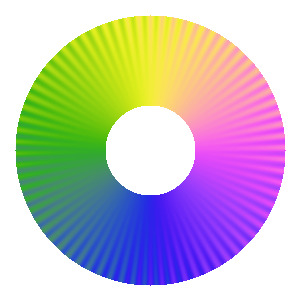
\includegraphics[width=4cm]{figures/C2_colourmap.jpg}
\\ C2 colourmap
\label{fig:C2_colourmap}
\end{figure*}

The \textit{C2} coloumap is also cyclic and useful for 3D magnetic systems such as vortex states. It has four principle directions of magenta, yellow, green and blue. As it is cyclic, there will be a smooth transition between colour at all angles, irrespective of what is chosen as the zero degree spin direction. Sytems which benefit from this colourmap may also use the \textit{3D} parameter which applies a brightness effect along the x-axis.

\vspace{5pt}
\begin{figure*}[!h]
\center

\includegraphics[width=7cm]{figures/BWR_colourmap.jpg}
\\ BWR colourmap
\label{fig:BWR_colourmap}
\end{figure*}

The \textit{BWR} colourmap is very similar in properties to the CBWR map however it is not cyclic. This mean that spins along the positive z-axis will be red with a small positive y-component and blue with a small negative y-component. There will be an immediate flip from bright red to blue as this transition occurs. This can be used to emphasise the transition between spin directions. The transition point can be changed by using \textit{vector-z}. 

\vspace{5pt}
\begin{figure*}[!h]
\center
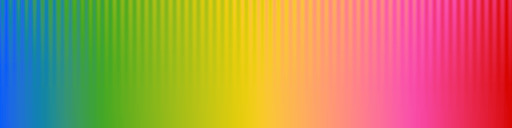
\includegraphics[width=7cm]{figures/Rainbow_colourmap.jpg}
\\ Rainbow colourmap
\label{fig:Rainbow_colourmap}
\end{figure*}

The \textit{Rainbow} colourmap can be used in 2D systems where spins are aligned in many different directions such as high temperature simulations. While it is still designed to be somewhat perceptually uniform, this is very difficult to do with rainbow palettes hence its use typically loses detail when compared to other maps, however it is also one of the most vibrant.

{\zicf custom-colourmap = filename }\phantomsection\addcontentsline{toc}{subsection}{custom-colourmap} A user defined colourmap can also be used. To apply a different map, a file containing 256 colours in the RBG format must be provided in the same directory that \vdc is run. RGB values must be space separated, with no other information such as line numbers. The beginning of an example colourmap is shown below. 

Pregenerated perceptually uniform colourmaps of various forms, including those included in vampire by default, can be found in \textit{peterkovesi.com/projects/\newline colourmaps/index.html} under the Download secion.

\subsection*{custom\_colourmap\_file}
{\footnotesize
\begin{verbatim}
0.000000 0.000000 0.000000
0.005561 0.005563 0.005563
0.011212 0.011219 0.011217
0.016877 0.016885 0.016883
0.022438 0.022448 0.022445
0.027998 0.028011 0.028008
0.033540 0.033554 0.033551
0.039316 0.039333 0.039329
0.044700 0.044719 0.044714
0.049695 0.049713 0.049709
0.054322 0.054343 0.054338
\end{verbatim}
}

{\zicf 3D = bool [default false]}\phantomsection\addcontentsline{toc}{subsection}{3D} POV-Ray images produced by \vdc can have a 3D brightening effect applied. Spins which do not line only in the yz-plane have their brightness adjusted according to their x-axis spin component.

{\zicf vector-z = float vector(3) [default \{0,0,1\}]}\phantomsection\addcontentsline{toc}{subsection}{vector-z} The principle axis, along which colour is applied, is the z-axis. This determines where colours will occur depending on the colourmap being used. By default the \textit{CBWR} map is used; spins along the positive z-direction are red, those along the negative z-direction are blue, and spins aligned along the xy-plane are white.

In many cases, the overall magnetic moment does not necessarily lie along the z-axis. To remedy this, a new \textit{vector-z} may be defined. To redefine the z-axis, use the parameter \textit{vector-z} followed by a direction vector. This does not need to be normalised.

For example, if the user defines \textit{vector-z} = \{1,1,1\}, spins along the \{1,1,1\} direction will be red, \{-1,-1,-1\} will be blue and those perpendicular to the given axis will be white. Brackets can be omitted.

{\zicf vector-x = float vector(3) [default \{0,0,1\}]}\phantomsection\addcontentsline{toc}{subsection}{vector-x} In some cases, the colourmap may not be symmetric along the default xy-plane, such as the \textit{C2} colourmap. Here, spins along positive-y are magenta, while those antiparallel are green. This can be adjusted using a similar command line argument \textit{vector-x}, however this argument cannot be used without first defining \textit{vector-z}. 

{\zicf afm = int [one or more values] }\phantomsection\addcontentsline{toc}{subsection}{afm} POV-Ray visualization of antiferromagnets can be difficult due to the contrast of colours of antiparallel spins. To remedy this, it is possible to define materials as antiferromagnetic. These materials will have their colours flipped so that they match neighbouring spins while their spin direction remains antiferromagnetic.

\section*{Micromagnetic visualization with POV-Ray}
\phantomsection\addcontentsline{toc}{section}{Micromagnetic visualization with POV-Ray}
cell2povray

macros

customization

colouring options

\section*{Visualization Movies}
\phantomsection\addcontentsline{toc}{section}{Visualization Movies}
